\documentclass[11pt,a4paper]{article}
\usepackage[a4paper,margin=2.1cm]{geometry}
\usepackage[T1]{fontenc}
\usepackage{newtxtext,newtxmath}
\usepackage{microtype}
\usepackage{graphicx}
\usepackage{booktabs}
\usepackage[table]{xcolor}
\usepackage{amsmath}
\usepackage{caption}
\usepackage{enumitem}
\usepackage{float}
\usepackage{needspace}
\usepackage[section]{placeins}
\usepackage[round]{natbib}
\usepackage[colorlinks=true,linkcolor=blue!50!black,citecolor=blue!50!black,urlcolor=blue!50!black]{hyperref}
\usepackage{titlesec}
\titlespacing*{\section}{0pt}{1.1ex plus .4ex}{.6ex}
\titlespacing*{\subsection}{0pt}{.9ex plus .3ex}{.4ex}
\setlist{itemsep=1pt,topsep=2pt,parsep=0pt}
\captionsetup{font=small,labelfont=bf,skip=3pt}
\setlength{\textfloatsep}{8pt plus 2pt}
\setlength{\floatsep}{6pt plus 2pt}
\setlength{\intextsep}{6pt plus 2pt}
\graphicspath{{generated/}{../outputs/task2/figures/}{../outputs/task3/figures/}}
% generated by report/make_tables.py -- do not edit
\newcommand{\ANCoverPct}{29.3}
\newcommand{\ANCovered}{5,727}
\newcommand{\ANTotal}{19,544}
\newcommand{\AbttWSMax}{0.71}
\newcommand{\AbttWSMin}{0.64}
\newcommand{\AnisoLstar}{0.29}
\newcommand{\AnisoLzero}{0.04}
\newcommand{\AnisoMax}{0.40}
\newcommand{\AnisoMaxLayer}{11}
\newcommand{\AucChain}{0.75}
\newcommand{\AucCtx}{0.70}
\newcommand{\AucProbe}{0.96}
\newcommand{\AucTOne}{0.54}
\newcommand{\AucTThree}{0.46}
\newcommand{\BestAnAcc}{80.3}
\newcommand{\BestAnLayer}{2}
\newcommand{\BestSemLayer}{1}
\newcommand{\BestSemWS}{0.690}
\newcommand{\ChainMST}{43.2}
\newcommand{\ChainPool}{43.0}
\newcommand{\ConcatAN}{22.2}
\newcommand{\ConcatWS}{0.397}
\newcommand{\ExCtx}{33}
\newcommand{\ExProbe}{83}
\newcommand{\ExTOne}{25}
\newcommand{\ExTThree}{25}
\newcommand{\ExText}{Your children will be taken care of and loved by a professional staff.}
\newcommand{\FeatGB}{5.1}
\newcommand{\FeatSeconds}{410}
\newcommand{\FnDegGold}{1.05}
\newcommand{\FnDegTOne}{1.84}
\newcommand{\FnDegTThree}{2.29}
\newcommand{\GoldSameUpos}{0.13}
\newcommand{\GoldSameUposNon}{0.09}
\newcommand{\LadConcatMST}{19.2}
\newcommand{\LadConcatPool}{25.1}
\newcommand{\LadCtxMST}{35.9}
\newcommand{\LadCtxPool}{38.2}
\newcommand{\LadProjMST}{29.5}
\newcommand{\LadProjPool}{35.9}
\newcommand{\LinDSpr}{0.549}
\newcommand{\LinNSpr}{0.333}
\newcommand{\LinRoot}{29.4}
\newcommand{\LinUUAS}{43.1}
\newcommand{\LitDspr}{0.760}
\newcommand{\LitLstar}{8}
\newcommand{\LitNspr}{0.803}
\newcommand{\LitRoot}{58.6}
\newcommand{\LitUuas}{62.0}
\newcommand{\Lstar}{8}
\newcommand{\LstarRank}{128}
\newcommand{\LtwelveUUAS}{67.6}
\newcommand{\LzeroAn}{72.1}
\newcommand{\LzeroUUAS}{58.7}
\newcommand{\LzeroWS}{0.685}
\newcommand{\MSTPool}{660}
\newcommand{\MaxDegGold}{4.53}
\newcommand{\MaxDegTThree}{5.46}
\newcommand{\MaxWP}{335}
\newcommand{\NDevSents}{2,001}
\newcommand{\NDevTokens}{25,148}
\newcommand{\NNCoocRandom}{0.07}
\newcommand{\NNCoocTOne}{0.56}
\newcommand{\NNCoocTThree}{0.16}
\newcommand{\NNSameRandom}{0.22}
\newcommand{\NNSameTOne}{0.33}
\newcommand{\NNSameTThree}{0.74}
\newcommand{\NTestSents}{2,077}
\newcommand{\NTestTokens}{25,094}
\newcommand{\NTrainSents}{12,544}
\newcommand{\NTrainTokens}{204,578}
\newcommand{\PRelAmod}{0.87}
\newcommand{\PRelAux}{0.89}
\newcommand{\PRelCase}{0.73}
\newcommand{\PRelCc}{0.82}
\newcommand{\PRelCompound}{0.87}
\newcommand{\PRelConj}{0.56}
\newcommand{\PRelDet}{0.91}
\newcommand{\PRelMark}{0.80}
\newcommand{\PRelNsubj}{0.84}
\newcommand{\PRelObj}{0.93}
\newcommand{\PRelObl}{0.69}
\newcommand{\PRelZeroAmod}{0.76}
\newcommand{\PRelZeroAux}{0.83}
\newcommand{\PRelZeroCase}{0.35}
\newcommand{\PRelZeroCc}{0.40}
\newcommand{\PRelZeroCompound}{0.82}
\newcommand{\PRelZeroConj}{0.38}
\newcommand{\PRelZeroDet}{0.61}
\newcommand{\PRelZeroMark}{0.56}
\newcommand{\PRelZeroNsubj}{0.62}
\newcommand{\PRelZeroObj}{0.73}
\newcommand{\PRelZeroObl}{0.42}
\newcommand{\PtANOnlyA}{3,848}
\newcommand{\PtANOnlyB}{0}
\newcommand{\PtAbttANA}{276}
\newcommand{\PtAbttANB}{88}
\newcommand{\PtAbttWSDiff}{+0.105}
\newcommand{\PtMSTCI}{[$-$6.4, 3.2]}
\newcommand{\PtMSTDiff}{$-$2.1}
\newcommand{\PtPoolCI}{[$-$8.0, $-$5.8]}
\newcommand{\PtPoolDiff}{$-$6.9}
\newcommand{\PtWSCI}{[0.36, 0.61]}
\newcommand{\PtWSDiff}{+0.474}
\newcommand{\QGoodMissed}{none}
\newcommand{\QGoodSpurious}{none}
\newcommand{\QGoodText}{I have eaten here several times and everytime the service is slower than slow.}
\newcommand{\QGoodUUAS}{1.00}
\newcommand{\QPoorMissed}{Raleigh-Chicago (conj), Raleigh-Seoul (conj), to-Chicago (case), Chicago-Seoul (nmod), to-Seoul (case), and-Seoul (cc), to-Manila (case)}
\newcommand{\QPoorSpurious}{Raleigh-to, to-to, Chicago-Chicago, Chicago-Seoul, Chicago-Seoul, to-to, and-then}
\newcommand{\QPoorText}{Raleigh to Chicago, Chicago to Seoul and then Seoul to Manila.}
\newcommand{\QPoorUUAS}{0.30}
\newcommand{\QTypicalMissed}{Say-finished (discourse), finished-found (conj)}
\newcommand{\QTypicalSpurious}{Say-after, I-I}
\newcommand{\QTypicalText}{Say after I finished those 2 years and I found a job.}
\newcommand{\QTypicalUUAS}{0.82}
\newcommand{\RandomMST}{15.2}
\newcommand{\RandomPool}{17.1}
\newcommand{\RankANSpr}{0.855}
\newcommand{\RankAUUAS}{77.4}
\newcommand{\RankBNSpr}{0.859}
\newcommand{\RankBUUAS}{79.2}
\newcommand{\RankCNSpr}{0.859}
\newcommand{\RankCUUAS}{79.5}
\newcommand{\SkewTOne}{2.10}
\newcommand{\SkewTThree}{1.45}
\newcommand{\StaticMSTMax}{21}
\newcommand{\StaticMSTMin}{15}
\newcommand{\TOneANCorrect}{29}
\newcommand{\TOneANCov}{0.51}
\newcommand{\TOneANFull}{0.15}
\newcommand{\TOneANSem}{2.1}
\newcommand{\TOneANSyn}{0.26}
\newcommand{\TOneMST}{20.5}
\newcommand{\TOneMSTCI}{[16.3, 26.2]}
\newcommand{\TOneMSTEdges}{234}
\newcommand{\TOnePool}{24.8}
\newcommand{\TOneRelAdvmod}{0.36}
\newcommand{\TOneRelAmod}{0.40}
\newcommand{\TOneRelCase}{0.12}
\newcommand{\TOneRelCc}{0.05}
\newcommand{\TOneRelConj}{0.34}
\newcommand{\TOneRelDet}{0.14}
\newcommand{\TOneRelMark}{0.13}
\newcommand{\TOneRelNsubj}{0.23}
\newcommand{\TOneRelObj}{0.31}
\newcommand{\TOneVsChain}{$-$22.6}
\newcommand{\TOneVsChainCI}{[$-$27.0, $-$16.9]}
\newcommand{\TOneVsRandom}{+5.3}
\newcommand{\TOneVsRandomCI}{[1.4, 9.2]}
\newcommand{\TOneWSCI}{[$-$0.03, 0.22]}
\newcommand{\TOneWSCov}{0.104}
\newcommand{\TOneWSFreqFive}{0.248}
\newcommand{\TOneWSFreqFiveN}{128}
\newcommand{\TOneWSFreqTen}{0.283}
\newcommand{\TOneWSFreqTenN}{75}
\newcommand{\TOneWSFreqTwenty}{0.317}
\newcommand{\TOneWSFreqTwentyN}{32}
\newcommand{\TOneWSFull}{0.048}
\newcommand{\TThreeAANCov}{71.0}
\newcommand{\TThreeAANFull}{20.8}
\newcommand{\TThreeAANSem}{79.0}
\newcommand{\TThreeAANSyn}{69.7}
\newcommand{\TThreeAMST}{19.7}
\newcommand{\TThreeAMSTCI}{[14.9, 26.2]}
\newcommand{\TThreeANCov}{67.7}
\newcommand{\TThreeANFull}{19.8}
\newcommand{\TThreeANSem}{74.5}
\newcommand{\TThreeANSyn}{66.6}
\newcommand{\TThreeAPool}{19.6}
\newcommand{\TThreeAWSCI}{[0.61, 0.74]}
\newcommand{\TThreeAWSCov}{0.682}
\newcommand{\TThreeAWSFreqTwenty}{0.724}
\newcommand{\TThreeAWSFull}{0.539}
\newcommand{\TThreeCapital}{93.6}
\newcommand{\TThreeCurrency}{0/28}
\newcommand{\TThreeMST}{18.4}
\newcommand{\TThreeMSTCI}{[13.6, 26.0]}
\newcommand{\TThreeOpposite}{26.9}
\newcommand{\TThreePlural}{96.6}
\newcommand{\TThreePool}{17.9}
\newcommand{\TThreeRelAmod}{0.16}
\newcommand{\TThreeRelConj}{0.44}
\newcommand{\TThreeRelDet}{0.30}
\newcommand{\TThreeRelMark}{0.35}
\newcommand{\TThreeRelNsubj}{0.09}
\newcommand{\TThreeRelObj}{0.15}
\newcommand{\TThreeRelObl}{0.09}
\newcommand{\TThreeWSCI}{[0.47, 0.66]}
\newcommand{\TThreeWSCov}{0.577}
\newcommand{\TThreeWSFreqTwenty}{0.661}
\newcommand{\TThreeWSFull}{0.452}
\newcommand{\TTwoRefMST}{81.2}
\newcommand{\TTwoRefPool}{82.9}
\newcommand{\TestOOV}{7.5}
\newcommand{\TiedLayers}{6--8}
\newcommand{\TtwoDevDspr}{0.826}
\newcommand{\TtwoDevNspr}{0.855}
\newcommand{\TtwoDevRoot}{87.2}
\newcommand{\TtwoDevUuas}{80.0}
\newcommand{\TtwoTestArgmax}{6}
\newcommand{\TtwoTestDspr}{0.822}
\newcommand{\TtwoTestNspr}{0.859}
\newcommand{\TtwoTestRoot}{87.5}
\newcommand{\TtwoTestUuas}{79.5}
\newcommand{\VocabSingletonPct}{47}
\newcommand{\VocabSingletons}{7,789}
\newcommand{\VocabTypes}{16,654}
\newcommand{\WSCoverPct}{70.3}
\newcommand{\WSCovered}{248}
\newcommand{\WSMedianCount}{11}

% generated by report_combined/make_combined.py
\newcommand{\ALitUUASonetwoeight}{62.0}
\newcommand{\ANSprthirtytwo}{0.855}
\newcommand{\ASweepMST}{19.8}
\newcommand{\ASweepMSTLayer}{10}
\newcommand{\AUUASthirtytwo}{77.4}
\newcommand{\BANAll}{0.15}
\newcommand{\BANCov}{0.85}
\newcommand{\BChainFull}{40.5}
\newcommand{\BChainTwenty}{35.5}
\newcommand{\BDSpr}{0.784}
\newcommand{\BDevUUAS}{67.2}
\newcommand{\BEdgesTwenty}{282}
\newcommand{\BFullEdges}{23,017}
\newcommand{\BFullSents}{1,926}
\newcommand{\BMSTFull}{17.8}
\newcommand{\BMSTTwenty}{16.7}
\newcommand{\BNSpr}{0.802}
\newcommand{\BNoVecFull}{11.5}
\newcommand{\BNoVecTwenty}{7.4}
\newcommand{\BRandFull}{14.3}
\newcommand{\BRandTwenty}{13.1}
\newcommand{\BRoot}{72.4}
\newcommand{\BSweepAN}{86.2}
\newcommand{\BSweepMST}{16.0}
\newcommand{\BSweepWS}{0.723}
\newcommand{\BTAllAN}{67.7}
\newcommand{\BTAllFull}{14.7}
\newcommand{\BTAllMST}{9.9}
\newcommand{\BTAllWS}{0.577}
\newcommand{\BTCenAN}{78.3}
\newcommand{\BTCenFull}{16.0}
\newcommand{\BTCenMST}{13.5}
\newcommand{\BTCenWS}{0.706}
\newcommand{\BTPcaAN}{81.4}
\newcommand{\BTPcaFull}{15.5}
\newcommand{\BTPcaMST}{13.5}
\newcommand{\BTPcaWS}{0.678}
\newcommand{\BTSameAN}{77.1}
\newcommand{\BTSameFull}{14.5}
\newcommand{\BTSameMST}{9.6}
\newcommand{\BTSameWS}{0.648}
\newcommand{\BUUAS}{66.4}
\newcommand{\BUUASnp}{68.9}
\newcommand{\BVocab}{8,865}
\newcommand{\BWSAllZero}{0.024}
\newcommand{\BWSCov}{0.189}
\newcommand{\LitMinEpoch}{1}
\newcommand{\XSubN}{203}
\newcommand{\XTOneAllZero}{0.060}
\newcommand{\XTOneSub}{0.171}
\newcommand{\XTThreeAAllZero}{0.420}
\newcommand{\XTThreeASub}{0.716}
\newcommand{\XTThreeAllZero}{0.288}
\newcommand{\XTThreeSub}{0.648}

\newcommand{\lstar}{\ensuremath{\ell^*}}
\newcommand{\pt}{\,pt}
\newcommand{\blk}[1]{\par\needspace{5\baselineskip}\smallskip\noindent\textbf{#1}\par\nobreak\vspace{1pt}}
\setlist[itemize]{leftmargin=1.3em,itemsep=1pt,topsep=2pt,parsep=0pt}
\setlist[enumerate]{leftmargin=1.5em,itemsep=1pt,topsep=2pt,parsep=0pt}
% ---- fill in the teammate's details here ----
\newcommand{\TeammateName}{Trishita Saha}
\newcommand{\TeammateRoll}{26CS91R13}

\title{\vspace{-1.2cm}\textbf{From Static to Contextual: Distributional Semantics and What's Inside BERT}\\[2pt]
\large Combined report: two independent implementations compared\\[1pt]
\normalsize NLP CS60075 Assignment II -- Project 5, dataset: UD English EWT}
\author{Yellapu Dheeraj Babu (23CS10081) \qquad \TeammateName{} (\TeammateRoll)}
\date{November 2026}

\begin{document}
\maketitle
\vspace{-0.6cm}
\begin{abstract}
\noindent The two of us implemented the project independently and compare the two implementations here: \textbf{A}
(Y.\,D.\,Babu) and \textbf{B} (\TeammateName). The project builds PPMI+SVD vectors from UD English EWT (Task~1), reproduces the
\citet{hewitt} structural probe on \texttt{bert-base-uncased} (Task~2), and pools the most syntactic layer into static vectors
(Task~3). \textbf{Both implementations find the same best layer (\lstar=8) and the same qualitative picture.} BERT-static vectors are far
better than PPMI-SVD on WordSim-353 and analogies, but no better (in fact worse) on the tree-recovery check, so the semantic and
syntactic evaluations disagree. Under identical settings the two Task~3 pipelines give \emph{the same numbers to three decimals}.
The one large quantitative difference is the probe's UUAS (A \TtwoTestUuas\%, B \BUUASnp\%, paper 79.8\%). We trace it to the training
schedule: B uses a constant learning rate, A uses the paper's decay. A control run in A with B's schedule shows the same drop (\ALitUUASonetwoeight\% when the last epoch is kept), and
the schedule also changes which probe rank looks best.
\end{abstract}

% =====================================================================================================
\needspace{11\baselineskip}\section{Introduction}
Count-based distributional models give one fixed vector per word \citep{levy2014}; BERT \citep{devlin} gives every token a
context-dependent vector. On UD English EWT \citep{silveira,ud} the project asks:
\begin{itemize}
\item \textbf{T1:} how good are PPMI+SVD vectors from 200k words?
\item \textbf{T2:} which BERT layer encodes dependency trees best, according to a structural probe?
\item \textbf{T3:} if that layer is averaged into static vectors, are they better than T1 on meaning and on tree structure -- and do
the two answers agree?
\item \textbf{Ours, because we implemented everything twice:} which conclusions survive a change of implementation?
\end{itemize}

\blk{Summary of the comparison}
\begin{itemize}
\item \textbf{Robust (both implementations agree):}
\begin{itemize}
\item \lstar=8 with a mid-layer peak;
\item T3 $\gg$ T1 on WordSim-353 and analogies;
\item T3 $<$ T1 on the MST check, close to a random tree;
\item the best layers for static semantics are 1--2, not \lstar;
\item mean-centring / all-but-the-top helps T3.
\end{itemize}
\item \textbf{Implementation-sensitive:}
\begin{itemize}
\item the absolute probe UUAS and the best probe rank (training schedule);
\item T1's WordSim $\rho$ (vocabulary cut-off and pair subset);
\item absolute MST levels (sentence sample and punctuation handling).
\end{itemize}
\end{itemize}

% =====================================================================================================
\needspace{11\baselineskip}\section{Data and the two implementations}\label{sec:impl}
\blk{Shared by both implementations}
\begin{itemize}
\item EWT splits: 12,544 / 2,001 / 2,077 sentences; 204,578 train tokens; 16,654 lowercased types.
\item Benchmarks: WordSim-353 \citep{ws353} and Google analogies \citep{mikolov}, gensim copies.
\item Model: frozen \texttt{bert-base-uncased}; a word's vector = mean of its word pieces.
\item The paper's probes and L1 losses; \lstar{} selected on dev.
\end{itemize}
Table~\ref{tab:impl} lists every choice in which the two implementations differ.

\begin{table}[h]\centering\footnotesize\setlength{\tabcolsep}{4pt}
\begin{tabular}{p{0.20\textwidth}p{0.37\textwidth}p{0.37\textwidth}}
\toprule
 & \textbf{A} (Y.\,D.\,Babu) & \textbf{B} (\TeammateName) \\
\midrule
EWT loading & HF \texttt{universal\_dependencies}, pinned tag \texttt{ud2.18-loader-v2.3.0} & official \texttt{.conllu} files, GitHub \texttt{master} branch (HF loader failed for B) \\
T1 vocabulary & all 16,654 types (min.\ count 1) & 8,865 types with count $\ge$2; rarer words dropped \\
SVD & sklearn \texttt{TruncatedSVD}, randomized, seed 42 & scipy \texttt{svds}, fixed start vector \\
WS-353 ``all 353'' & OOV pair $\to$ median model similarity & OOV pair $\to$ similarity 0 \\
Analogy coverage & 5,727 covered questions & 3,406 covered questions \\
20-sentence sample & seed 42; 5--40 non-punct.\ words, \emph{all in vocabulary}; punctuation excluded (234 edges) & seed 42; $\ge$5 tokens, any words; \emph{punctuation included}; OOV words at distance 1 (282 edges) \\
Random-tree baseline & uniformly random spanning tree (expected UUAS) & MST of random distances (100 draws) \\
Robustness set & all 660 eligible test sentences & all 1,926 multi-token test sentences \\
Probed layers & 0 (embeddings) + 1--12; 78 probes & 1--12; 72 probes \\
\textbf{Probe schedule} & Adam 1e-3, 30 ep., \textbf{lr $\times$0.1 when dev loss stalls} (paper), best-dev checkpoint & Adam 1e-3, 30 ep., \textbf{constant lr}, best-dev checkpoint \\
UUAS punctuation & excluded (paper convention) & reported with and without \\
Depth Spearman & per-length average, macro over lengths 5--50 (paper) & per-sentence mean over lengths 5--50 \\
T3 vocabulary & all 16,654 types & main: T1's 8,865 types; variant: all types \\
Anisotropy fix & all-but-the-top, $D=7$ \citep{mu}; also on T1 & mean-centring; centring + PCA to 100 dims \\
Uncertainty & bootstrap CIs, paired bootstrap / McNemar tests & micro and macro averages; full test split \\
Seeds & 42 everywhere; probe $42+1000\ell+k$ (+500 depth) & sample 42; SVD start 0; probe $1000k$ (+7 depth) + layer \\
\bottomrule
\end{tabular}
\caption{Where implementations A and B differ (everything else is shared). B's entries were checked against B's source code (\texttt{Codes/*.py}).}\label{tab:impl}\end{table}

\blk{Cross-check: same settings give the same numbers (Table~\ref{tab:cross})}
\begin{itemize}
\item B's raw outputs are not available to us, so A's outputs were re-scored under B's settings.
\item Every Task~3 number of B that can be reproduced this way is reproduced \textbf{exactly}: the two pooling and evaluation
pipelines are equivalent.
\item The T1 numbers differ only because B's vectors were trained on the count-$\ge$2 vocabulary.
\end{itemize}
\begin{table}[h]\centering\footnotesize\begin{tabular}{lccl}
\toprule
quantity & A (recomputed in B's setting) & B (reported) & \\
\midrule
train / dev / test sentences & 12,544 / 2,001 / 2,077 & 12,544 / 2,001 / 2,077 & identical \\
train tokens; lowercased types & 204,578; 16,654 & 204,578; 16,654 & identical \\
types with count $\ge$2 (B's T1 vocabulary) & 8,865 & 8,865 & identical \\
analogy questions, all words count $\ge$2 & 3,406 & 3,406 & identical \\
T3 layer 8, WS-353 $\rho$ on those 203 pairs & 0.648 & 0.648 & identical \\
T3 layer 8 (all types), WS $\rho$, 248 covered pairs & 0.577 & 0.577 & identical \\
T3 layer 8 (all types), WS $\rho$, all 353, missing $=0$ & 0.288 & 0.288 & identical \\
T3 layer 8 (all types), analogy, 5,727 covered & 67.7 & 67.7 & identical \\
\quad semantic / syntactic & 74.5 / 66.6 & 74.5 / 66.6 & identical \\
T3 layer 8 (all types), analogy, all 19,544 & 19.8 & 19.8 & identical \\
T1, WS $\rho$ on the 203 pairs & 0.171$^a$ & 0.189$^b$ & vocabulary cut-off \\
T1, WS $\rho$, all 353, missing $=0$ & 0.060$^a$ & 0.024$^b$ & vocabulary cut-off \\
\bottomrule
\end{tabular}

\caption{A's outputs re-scored in B's setting vs.\ B's reported numbers. $^a$A's vectors (min.\ count 1); $^b$B's vectors (count $\ge$2), so the
T1 rows compare two different vector sets on the same pairs.}\label{tab:cross}\end{table}

% =====================================================================================================
\needspace{11\baselineskip}\section{Task 1 -- PPMI + SVD}\label{sec:t1}
\blk{Method (both)}
\begin{itemize}
\item Symmetric $\pm$5-word co-occurrence matrix over the training sentences; PPMI \citep{levy2014}; top 100 SVD dimensions, vectors $U\Sigma$.
\item Cosine similarity; analogies by the vector offset with the three query words excluded.
\end{itemize}
\begin{table}[h]\centering\footnotesize\begin{tabular}{lll}
\toprule
Task 1 & A & B \\
\midrule
vocabulary & all 16,654 train types & 8,865 types (count $\ge$2) \\
WS-353 $\rho$, covered pairs & 0.104 (248) & 0.189 (203) \\
WS-353 $\rho$, all 353 & 0.048 (median) / 0.060 (zero) & 0.024 (zero) \\
analogy acc., covered & 0.51\% (5,727) & 0.85\% (3,406) \\
\quad semantic / syntactic & 2.1 / 0.26\% & 2.0 / 0.70\% \\
analogy acc., all 19,544 & 0.15\% & 0.15\% \\
MST UUAS, 20 sentences & 20.5 (234 edges) & 16.7 (282 edges) \\
\quad random tree / linear chain & 15.2 / 43.2 & 13.1 / 35.5 \\
MST UUAS, robustness set & 24.8 (660 sent.) & 17.8 (1,926 sent.) \\
\quad random tree / linear chain & 17.1 / 43.0 & 14.3 / 40.5 \\
\bottomrule
\end{tabular}

\caption{Task 1 in both implementations (numbers in brackets: covered items / sentences or edges).}\label{tab:t1}\end{table}

\blk{Agreement}
\begin{itemize}
\item Both find weak, data-limited vectors: WS-353 $\rho$ near 0 over all 353 pairs and analogies below 1\%.
\item In both, the MST beats a random tree but stays well below the linear chain.
\end{itemize}

\blk{Differences explained}
\begin{enumerate}
\item \textbf{B's higher covered $\rho$} (\BWSCov{} vs.\ \TOneWSCov) has two causes:
\begin{itemize}
\item \emph{different pairs} -- B's 203 covered pairs exclude words seen once; A's vectors score \XTOneSub{} on those same pairs, so most of
the gap is the subset (consistent with A's frequency analysis: $\rho$ \TOneWSFreqTwenty{} on pairs of words seen $\ge$20 times);
\item \emph{different vectors} -- dropping singletons removes noisy rows and contexts before the SVD (\XTOneSub{} $\to$ \BWSCov).
\end{itemize}
\item \textbf{``All 353'' numbers} differ by the imputation rule: with B's ``missing $=0$'' rule A gets \XTOneAllZero{} (B \BWSAllZero); with the
median rule A gets \TOneWSFull.
\item \textbf{MST levels} differ because B's sample keeps OOV words (at distance 1) and punctuation, which lowers every system and both
baselines (B: random \BRandTwenty, chain \BChainTwenty; A: \RandomMST, \ChainMST). The ordering random $<$ T1 $<$ chain is the same in both.
\end{enumerate}

\blk{Extra analyses (A)}
\begin{itemize}
\item \textbf{Levy et al.\ hyper-parameters} \citep{levy2015} (Table~\ref{tab:t1abl}): no setting rescues the analogies; the best variant
($p=0$) only reaches $\rho=0.134$ -- the limit is the 200k-word corpus.
\item \textbf{Per relation:} PPMI-SVD recovers content-word relations that co-occur (amod \TOneRelAmod, conj \TOneRelConj) and almost no
function-word attachments (case \TOneRelCase, det \TOneRelDet).
\end{itemize}
\begin{table}[h]\centering\footnotesize\setlength{\tabcolsep}{4pt}\begin{tabular}{lccccccc}
\toprule
 & \multicolumn{3}{c}{WordSim-353 $\rho$} & \multicolumn{2}{c}{Analogy acc.\ (\%)} & \multicolumn{2}{c}{MST UUAS (\%)} \\
\cmidrule(lr){2-4}\cmidrule(lr){5-6}\cmidrule(lr){7-8}
PPMI-SVD variant & covered (248) [95\% CI] & all 353 & freq.\,$\ge$20 & covered & all & 20 sent. & pool (660) \\
\midrule
\textbf{spec}: $\alpha{=}1$, $p{=}1$ (U$\Sigma$) & 0.104 [$-$0.03, 0.22] & 0.048 & 0.317 & 0.51 & 0.15 & 20.5 & 24.8 \\
$\alpha{=}0.75$, $p{=}1$ & 0.060 [$-$0.07, 0.20] & 0.043 & 0.199 & 0.65 & 0.19 & 15.8 & 20.8 \\
$\alpha{=}1$, $p{=}0.5$ & 0.129 [$-$0.00, 0.24] & 0.091 & 0.289 & 0.37 & 0.11 & 20.9 & 24.6 \\
$\alpha{=}1$, $p{=}0$ (U) & 0.134 [0.00, 0.25] & 0.089 & 0.320 & 0.21 & 0.06 & 22.6 & 24.5 \\
$\alpha{=}0.75$, $p{=}0.5$ & 0.097 [$-$0.04, 0.22] & 0.066 & 0.174 & 0.42 & 0.12 & 16.2 & 20.8 \\
spec + all-but-the-top ($D{=}1$) & 0.153 & 0.103 & 0.294 & 0.42 & -- & 20.5 & 24.5 \\
\midrule
linear chain (attach to next word) & -- & -- & -- & -- & -- & 43.2 & 43.0 \\
random tree (expected) & -- & -- & -- & -- & -- & 15.2 & 17.1 \\
\bottomrule
\end{tabular}

\caption{A's Task 1 with the Levy et al.\ variants ($\alpha$ = context-distribution smoothing, $p$ = eigenvalue weight) and baselines.}\label{tab:t1abl}\end{table}

% =====================================================================================================
\needspace{11\baselineskip}\section{Task 2 -- Structural probe}\label{sec:t2}
\blk{Method (both)}
\begin{itemize}
\item All layers of frozen \texttt{bert-base-uncased} extracted once (word = mean of its word pieces; fp16 cache).
\item Distance probe $\lVert B(h_i-h_j)\rVert^2$ and depth probe $\lVert Bh_i\rVert^2$; $B\in\mathbb{R}^{k\times768}$,
$k\in\{32,64,128\}$, $B\sim\mathcal{U}(-0.05,0.05)$; L1 loss normalised by $n^2$ / $n$.
\item Adam lr $10^{-3}$, batches of 20 sentences, 30 epochs, best-dev checkpoint; MST decoding; \lstar{} on dev UUAS.
\item \textbf{The decisive difference is the learning-rate schedule} (Table~\ref{tab:impl}).
\end{itemize}

\begin{figure}[t]\centering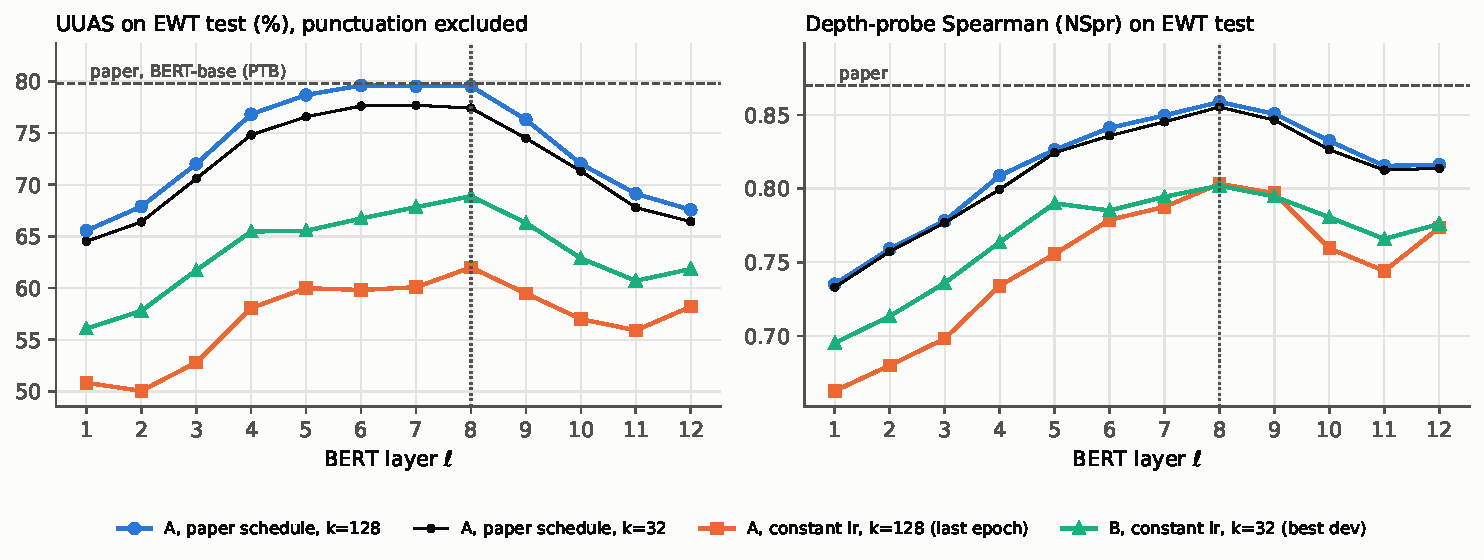
\includegraphics[width=\textwidth]{fig_layers_cmp.pdf}
\caption{Probe quality vs.\ layer in both implementations (EWT test). A's curves come from its outputs; B's from its Table~2. A's
constant-lr control (orange) uses B's schedule but keeps the last epoch; B (green) keeps the best dev epoch.}\label{fig:cmp}\end{figure}
\begin{table}[t]\centering\footnotesize\setlength{\tabcolsep}{3.8pt}\begin{tabular}{rccc|cc|cc|cc}
\toprule
 & \multicolumn{5}{c|}{UUAS (\%), punctuation excluded} & \multicolumn{4}{c}{depth Spearman (NSpr)} \\
 & \multicolumn{2}{c}{A, paper schedule} & A, const.\ lr & \multicolumn{2}{c|}{B, const.\ lr} & A, paper & A, const. & \multicolumn{2}{c}{B, const.\ lr} \\
$\ell$ & $k{=}32$ & $k{=}128$ & $k{=}128$, last ep. & $k{=}32$ & $k{=}128^\ast$ & $k{=}32$ & $k{=}128$ & $k{=}32$ & $k{=}128$ \\
\midrule
1 & 64.5 & 65.6 & 50.8 & 56.1 & 49.3$^\ast$ & 0.733 & 0.663 & 0.695 & 0.666 \\
2 & 66.4 & 67.9 & 50.1 & 57.8 & 51.4$^\ast$ & 0.757 & 0.680 & 0.713 & 0.647 \\
3 & 70.6 & 72.0 & 52.8 & 61.7 & 55.3$^\ast$ & 0.777 & 0.698 & 0.736 & 0.685 \\
4 & 74.8 & 76.8 & 58.1 & 65.5 & 58.2$^\ast$ & 0.799 & 0.734 & 0.764 & 0.712 \\
5 & 76.6 & 78.7 & 60.0 & 65.5 & 62.7$^\ast$ & 0.824 & 0.756 & 0.790 & 0.709 \\
6 & 77.6 & 79.6 & 59.8 & 66.7 & 63.0$^\ast$ & 0.836 & 0.779 & 0.785 & 0.718 \\
7 & 77.7 & 79.5 & 60.1 & 67.8 & 64.0$^\ast$ & 0.845 & 0.788 & 0.794 & 0.753 \\
\rowcolor{black!8} 8 & 77.4 & 79.5 & 62.0 & 68.9 & 64.5$^\ast$ & 0.855 & 0.803 & 0.802 & 0.757 \\
9 & 74.5 & 76.3 & 59.5 & 66.3 & 61.9$^\ast$ & 0.846 & 0.797 & 0.795 & 0.749 \\
10 & 71.3 & 72.0 & 57.0 & 62.9 & 57.0$^\ast$ & 0.826 & 0.760 & 0.780 & 0.715 \\
11 & 67.8 & 69.1 & 55.9 & 60.7 & 54.9$^\ast$ & 0.812 & 0.744 & 0.766 & 0.712 \\
12 & 66.4 & 67.6 & 58.2 & 61.9 & 54.2$^\ast$ & 0.814 & 0.773 & 0.776 & 0.752 \\
\bottomrule
\end{tabular}

\caption{Per-layer test results. $^\ast$B reports $k=128$ only with punctuation included. Shaded: \lstar=8.}\label{tab:t2}\end{table}
\begin{table}[t]\centering\footnotesize\begin{tabular}{lcccccc}
\toprule
system & $\ell^*$ & $k$ & UUAS & DSpr & NSpr & Root\% \\
\midrule
Paper: BERT-base (PTB WSJ, cased) & 7 (0-idx.) & full & 79.8 & 0.85 & 0.87 & 88.0 \\
A: paper schedule ($\times$0.1 lr decay, best dev) & 8 & 128 & 79.5 & 0.822 & 0.859 & 87.5 \\
A: constant lr, last epoch (control) & 8 & 128 & 62.0 & 0.760 & 0.803 & 58.6 \\
B: constant lr, best dev epoch & 8 & 32 & 68.9 & 0.784$^\dagger$ & 0.802$^\ddagger$ & 72.4 \\
\bottomrule
\end{tabular}

\caption{Best probes vs.\ \citet{hewitt} Table~1. UUAS excludes punctuation in all rows (B with punctuation: \BUUAS). $^\dagger$B's
distance Spearman; $^\ddagger$B averages per sentence, A per length (the paper's definition).}\label{tab:best}\end{table}

\blk{Agreement}
\begin{itemize}
\item Both pick \lstar=8.
\item Both see UUAS and depth Spearman rise to the middle layers and fall towards layer 12 (Fig.~\ref{fig:cmp}).
\item In both, the dev choice equals the test argmax or is statistically tied with it (A: layers \TiedLayers{} are tied by a paired bootstrap).
\end{itemize}

\blk{The UUAS gap is the schedule (A \TtwoTestUuas\%, B \BUUASnp\%, paper 79.8\%)}
\begin{enumerate}
\item \textbf{Control run:} A retrained with B's schedule (constant lr, last epoch, $k=128$) falls to \ALitUUASonetwoeight\%; B, with the same
schedule but best-dev selection, sits in between (\BUUASnp\%, Fig.~\ref{fig:cmp}).
\item \textbf{Same symptom:} B observes that the best dev epoch of $k=128$ distance probes is mostly epoch~1; in A's control the dev minimum is
also at epoch \LitMinEpoch, after which dev loss oscillates (0.54--0.59) for 29 epochs.
\item \textbf{Not over-fitting but non-convergence:} in A's control the \emph{training} loss also stays high (0.62 vs.\ 0.42 with decay).
With an L1 loss the gradient does not shrink near the optimum, so Adam's steps stay $\approx$lr and circle the minimum; the $\times$0.1
decay lets the probe settle.
\end{enumerate}

\blk{The schedule also reverses the rank conclusion}
\begin{itemize}
\item B (constant lr) finds $k=32$ best and reads it as over-fitting of larger probes.
\item A (decay) finds $k=128 \ge 64 > 32$ (at \lstar: \RankAUUAS{} / \RankBUUAS{} / \RankCUUAS\%), as the paper does.
\item The smaller probe is simply less hurt by non-convergence, so ``low rank generalises better'' is a property of the schedule, not of the data.
\item Both agree that the tree lives in a low-dimensional subspace: even $k=32$ is within about 2\pt{} of $k=128$ in A.
\end{itemize}

\blk{Remaining gap to the paper (A, $-$0.3\pt) and other observations}
\begin{itemize}
\item \textbf{Plausible causes (named by both):} 12.5k vs.\ $\approx$40k training sentences; web text vs.\ edited news; UD content-head trees
vs.\ Stanford Dependencies; uncased vs.\ cased BERT; rank $\le$128 and 30 epochs vs.\ full rank and up to 40 epochs.
\item \textbf{What context adds (A):} the layer-0 probe (\LzeroUUAS\%) matches the paper's non-contextual PROJ0 (59.8\%), so context adds
$\approx$21\pt{}, mostly for function words (case \PRelZeroCase$\to$\PRelCase, cc \PRelZeroCc$\to$\PRelCc).
\item \textbf{Easy and hard relations (A, Fig.~\ref{fig:rel}):} short head--dependent arcs are easy (obj \PRelObj, det \PRelDet, aux \PRelAux);
coordination (conj \PRelConj) and PP attachment (obl \PRelObl) are hard -- UD attaches every conjunct to the first, creating long arcs.
\item \textbf{Punctuation (B):} including it costs 2.5\pt{} (\BUUAS{} vs.\ \BUUASnp), because UD attaches punctuation to content heads.
\item \textbf{Root accuracy:} A \TtwoTestRoot\%, B \BRoot\% (B: 48--57\% for $k=128$), again consistent with the schedule effect.
\end{itemize}
\begin{figure}[t]\centering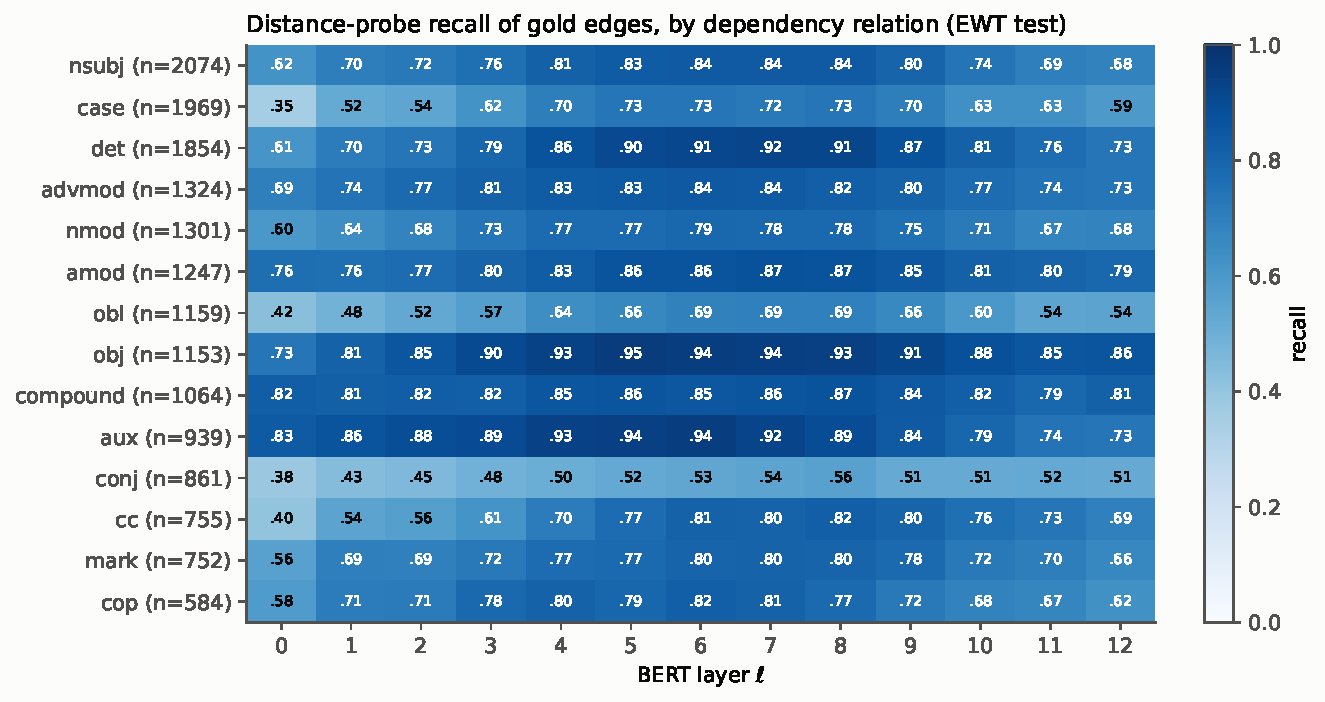
\includegraphics[width=0.78\textwidth]{relation_recall_heatmap.pdf}
\caption{A: probe recall of gold edges per dependency relation and layer (EWT test).}\label{fig:rel}\end{figure}

% =====================================================================================================
\needspace{11\baselineskip}\section{Task 3 -- BERT-derived static vectors}\label{sec:t3}
\blk{Method (both)}
\begin{itemize}
\item Average the layer-8 vectors of every training occurrence of a word type (mean over word pieces, then over occurrences) -- the
mean/mean pooling that \citet{bommasani} found best -- and evaluate with the Task~1 functions.
\item A evaluates all 16,654 types; B's main comparison restricts T3 to T1's 8,865 types (all types as a variant), so B's covered sets
are smaller.
\end{itemize}

\begin{table}[h]\centering\footnotesize\setlength{\tabcolsep}{4pt}\begin{tabular}{llcccc}
\toprule
 & & \multicolumn{2}{c}{WordSim-353 $\rho$} & \multicolumn{2}{c}{analogy accuracy (\%)} \\
\cmidrule(lr){3-4}\cmidrule(lr){5-6}
impl. & system & 248 covered & 203 (count $\ge$2) & covered & all 19,544 \\
\midrule
A & T1 PPMI-SVD & 0.104 (248) & 0.171 & 0.51 (5,727) & 0.15 \\
B & T1 PPMI-SVD (count $\ge$2) & -- & 0.189 & 0.85 (3,406) & 0.15 \\
\midrule A & T3 layer 8, all types & 0.577 (248) & 0.648 & 67.7 (5,727) & 19.8 \\
B & T3 layer 8, all types & 0.577 (248) & -- & 67.7 (5,727) & 19.8 \\
B & T3 layer 8, T1 vocabulary (main) & -- & 0.648 & 77.1 (3,406) & 13.4 \\
\midrule A & T3 + all-but-the-top ($D{=}7$) & 0.682 (248) & 0.716 & 71.0 (5,727) & 20.8 \\
B & T3 mean-centred (T1 vocab.) & -- & 0.706 & 78.3 (3,406) & 13.7 \\
B & T3 centred + PCA-100 (T1 vocab.) & -- & 0.678 & 81.4 (3,406) & 14.2 \\
\bottomrule
\end{tabular}

\caption{Semantic benchmarks. The ``203'' column scores every system on the same 203 pairs (A re-scored; Table~\ref{tab:cross}).
B's T1-vocabulary variants also restrict the analogy candidates to 8,865 words, which raises covered accuracy.}\label{tab:t3sem}\end{table}
\begin{table}[h]\centering\footnotesize\setlength{\tabcolsep}{4pt}\begin{tabular}{lcccc}
\toprule
 & \multicolumn{2}{c}{20 sampled sentences} & \multicolumn{2}{c}{robustness set} \\
\cmidrule(lr){2-3}\cmidrule(lr){4-5}
UUAS (\%) & A (234 edges) & B (282 edges) & A: 660 sent. & B: 1,926 sent. \\
\midrule
random tree & 15.2 & 13.1 & 17.1 & 14.3 \\
linear chain & 43.2 & 35.5 & 43.0 & 40.5 \\
\midrule T1 PPMI-SVD & 20.5 & 16.7 & 24.8 & 17.8 \\
T3 layer 8 (A: all types; B: T1 vocab.) & 18.4 & 9.6 & 17.9 & 14.5 \\
T3 layer 8, all types & 18.4 & 9.9 & 17.9 & 14.7 \\
T3 + anisotropy fix (A: ABTT; B: centred) & 19.7 & 13.5 & 19.6 & 16.0 \\
\midrule T2 probe, layer 8 (A only) & 81.2 & -- & 82.9 & -- \\
\bottomrule
\end{tabular}

\caption{Structural check (UUAS of the cosine-distance MST). The two implementations use different sentences (Table~\ref{tab:impl}), so
compare rows within a column.}\label{tab:t3struct}\end{table}

\blk{Meaning: both find a large, significant gain}
\begin{itemize}
\item \textbf{Same 203 pairs:} $\rho$ goes from \XTOneSub{} (A) / \BWSCov{} (B) to \XTThreeSub{} / \BTSameWS.
\item \textbf{Analogies:} from below 1\% to 68--77\% on covered questions.
\item \textbf{Significance (A):} $\Delta\rho=\PtWSDiff$ \PtWSCI; T3 solves \PtANOnlyA{} analogy questions T1 misses, T1 solves \PtANOnlyB{}
that T3 misses (Table~\ref{tab:tests}).
\item \textbf{Caveat (both):} not a data-matched comparison -- BERT brings pre-training on $\approx$3.3B words; EWT only supplies the contexts.
\item \textbf{Anisotropy:} removing the shared direction helps in both (A all-but-the-top \TThreeAWSCov; on the 203 pairs, B centring
\BTCenWS{} vs.\ A all-but-the-top \XTThreeASub), confirming that raw BERT vectors are anisotropic \citep{ethayarajh}.
\end{itemize}

\blk{Structure: both find no improvement}
\begin{itemize}
\item \textbf{20-sentence samples:} T3 below T1 in both (A \TThreeMST{} vs.\ \TOneMST; B \BTSameMST{} vs.\ \BMSTTwenty).
\item \textbf{Larger sets:} T3 below T1 in both (A \TThreePool{} vs.\ \TOnePool; B \BTSameFull{} vs.\ \BMSTFull), close to the random tree.
\item \textbf{Significance (A):} the 20-sentence difference is not significant ($\Delta=\PtMSTDiff$\pt, CI \PtMSTCI); the 660-sentence one is
($\Delta=\PtPoolDiff$\pt, CI \PtPoolCI). B reaches the same conclusion from its larger full-test set.
\item \textbf{So the two evaluations disagree -- in both implementations.}
\end{itemize}
\begin{table}[h]\centering\footnotesize\setlength{\tabcolsep}{4pt}\begin{tabular}{lccccc}
\toprule
 & WordSim-353 & \multicolumn{2}{c}{Analogy (McNemar)} & \multicolumn{2}{c}{MST $\Delta$UUAS (pt) [95\% CI]} \\
\cmidrule(lr){3-4}\cmidrule(lr){5-6}
A $-$ B & $\Delta\rho$ [95\% CI] & only A / only B & $p$ & 20 sentences & pool (660) \\
\midrule
T3 $-$ T1 & +0.474 [0.36, 0.61] & 3,848 / 0 & $<10^{-300}$ & $-$2.1 [$-$6.4, 3.2] & $-$6.9 [$-$8.0, $-$5.8] \\
T3+ABTT $-$ T1 & +0.579 [0.46, 0.71] & 4,036 / 0 & $<10^{-300}$ & $-$0.9 [$-$6.6, 5.6] & $-$5.1 [$-$6.2, $-$4.1] \\
T3+ABTT $-$ T3 & +0.105 [0.05, 0.16] & 276 / 88 & $1\times10^{-23}$ & +1.3 [$-$3.2, 5.6] & +1.7 [1.0, 2.6] \\
T2 probe $-$ T3 & -- & -- & -- & +62.8 [53.2, 69.6] & +65.0 [63.8, 66.3] \\
\bottomrule
\end{tabular}

\caption{A's paired tests on identical items (analogy: questions solved only by A / only by B, exact McNemar $p$).}\label{tab:tests}\end{table}

\blk{Layer sweep (both): the syntax layer is not the meaning layer (Fig.~\ref{fig:sweep})}
\begin{itemize}
\item \textbf{WordSim peaks at layer 1} in both (A \BestSemWS{} on 248 pairs, B \BSweepWS{} on 203), matching \citet{bommasani} (layer 1,
$\rho=0.683$ for bert-base-uncased with 10k contexts).
\item \textbf{Analogies peak at layer 2} in both (A \BestAnAcc\%, B \BSweepAN\%).
\item \textbf{Best static-MST layer is \ASweepMSTLayer{}} in both (A \ASweepMST\%, B \BSweepMST\%) -- still close to chance.
\item \textbf{Anisotropy (A):} raw WordSim falls with depth while anisotropy rises (\AnisoLzero{} $\to$ \AnisoMax); after all-but-the-top the
curve is almost flat (\AbttWSMin--\AbttWSMax), so much of the decline is the ``narrow cone'' effect.
\end{itemize}
\begin{figure}[t]\centering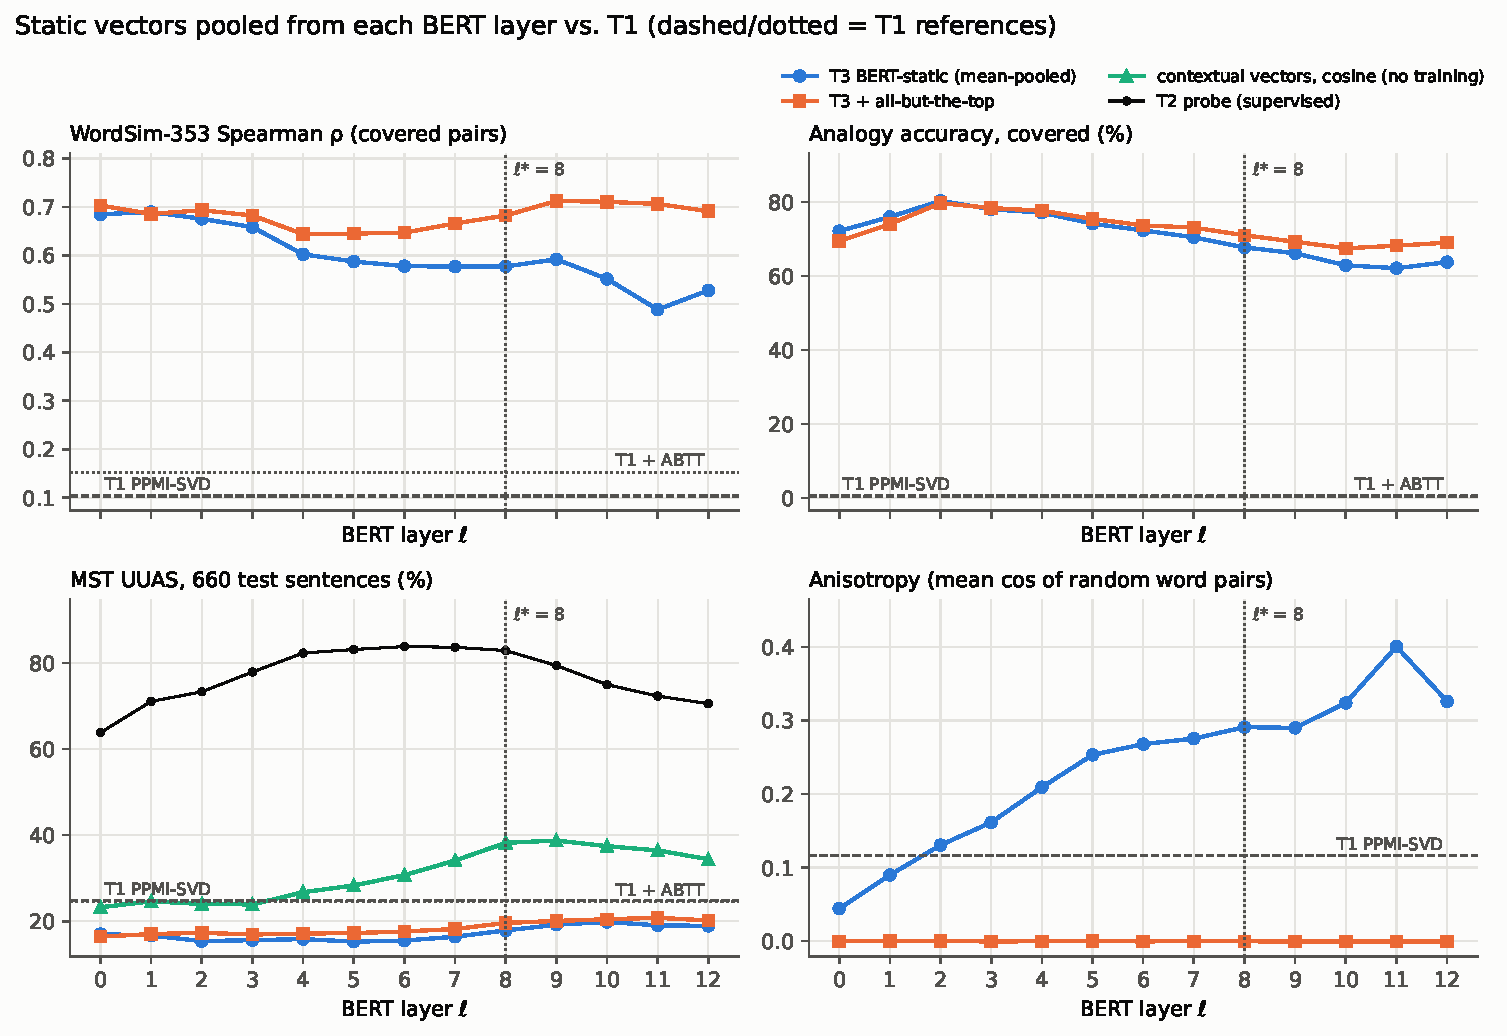
\includegraphics[width=0.92\textwidth]{layer_sweep.pdf}
\caption{A's layer sweep: static vectors pooled from each layer (raw and all-but-the-top) vs.\ T1; the MST panel also shows raw contextual
vectors and the probe on the same 660 sentences. B's sweep (its Fig.~2) has the same maxima: WordSim at layer 1, analogy at layer 2.}\label{fig:sweep}\end{figure}

% =====================================================================================================
\needspace{11\baselineskip}\section{Why the semantic and syntactic answers disagree}\label{sec:why}
B proposes three reasons; A tests each with a measurement (\texttt{diagnostics\_task3.py}, \texttt{extensions\_task3.py}).
\begin{enumerate}
\item \textbf{Pooling removes the context-dependent signal} (B).
\begin{itemize}
\item Measured by A's ladder on the same 660 sentences (Table~\ref{tab:ladder}): static T3 \TThreePool\% $\to$ the same vectors through the
probe's matrix $B$ \LadProjPool\% $\to$ per-token contextual vectors, plain cosine \LadCtxPool\% $\to$ trained probe \TTwoRefPool\%.
\end{itemize}
\item \textbf{The probe learns a projection; the MST check uses raw cosine} (B).
\begin{itemize}
\item Confirmed: even contextual vectors with raw cosine (\LadCtxPool\%) stay below the linear chain (\ChainPool\%).
\item The tree is in a learned low-rank subspace, not in the raw geometry.
\end{itemize}
\item \textbf{Edges join semantically dissimilar words; PPMI's window captures local co-occurrence} (B). A measured this as paradigmatic
vs.\ syntagmatic similarity \citep{sahlgren} (Table~\ref{tab:diag}):
\begin{itemize}
\item \textbf{T3 neighbours are substitutes:} \NNSameTThree{} share the word's part of speech (T1 \NNSameTOne; random \NNSameRandom).
\item \textbf{T1 neighbours are partners:} \NNCoocTOne{} co-occur with the word within $\pm$5 (T3 \NNCoocTThree; random \NNCoocRandom).
\item \textbf{Direct test, edge AUC} (does closeness predict attachment inside a sentence?): T3 \AucTThree{} (no information), T1 \AucTOne{}
(weakly informative), contextual \AucCtx, probe \AucProbe.
\item \textbf{Refinement:} gold edges are \emph{not} mostly between different parts of speech relative to non-edges (same-UPOS rate
\GoldSameUpos{} vs.\ \GoldSameUposNon), so the effect is about similarity, not word category.
\end{itemize}
\end{enumerate}
\blk{Further observations}
\begin{itemize}
\item \textbf{Hubs (A):} T3's MSTs are star-shaped around frequent function words (degree \FnDegTThree{} vs.\ gold \FnDegGold).
\item \textbf{OOV words (B):} \BNoVecTwenty\% of the words in B's sample have no vector and inject arbitrary distances; A's in-vocabulary
sample avoids this, and T3 is still below T1.
\end{itemize}
\begin{table}[h]\centering\footnotesize\setlength{\tabcolsep}{4pt}\begin{tabular}{llccc}
\toprule
representation for the MST & tier & 20 sentences [95\% CI] & pool (660) [95\% CI] & edge AUC \\
\midrule
random tree (expected) & -- & 15.2 & -- & -- \\
linear chain & -- & 43.2 [40.6, 46.4] & 43.0 [42.4, 43.7] & 0.75 \\
T1 PPMI-SVD (spec) & req. & 20.5 [16.3, 26.2] & 24.8 [23.7, 26.0] & 0.54 \\
T1 PPMI-SVD (p0) & B & 22.6 [17.8, 28.4] & 24.5 [23.4, 25.6] & -- \\
T3 BERT-static L8 & req. & 18.4 [13.6, 26.0] & 17.9 [16.8, 18.9] & 0.46 \\
T3 BERT-static L8 + ABTT & B & 19.7 [14.9, 26.2] & 19.6 [18.6, 20.7] & 0.44 \\
concat [T1 ; T3] (L2-normalised) & C & 19.2 [15.2, 25.1] & 25.1 [24.0, 26.2] & -- \\
T3 BERT-static L8 through probe B & C & 29.5 [23.7, 38.2] & 35.9 [34.3, 37.5] & -- \\
contextual L8, cosine (no training) & B & 35.9 [32.1, 39.6] & 38.2 [37.3, 39.2] & 0.70 \\
T2 distance probe L8 k=128 & ref. & 81.2 [75.9, 85.9] & 82.9 [81.9, 83.9] & 0.96 \\
\bottomrule
\end{tabular}

\caption{A's diagnostic ladder on the same sentences; edge AUC = probability that a gold edge pair is closer than a non-edge pair in the same sentence.}\label{tab:ladder}\end{table}
\begin{table}[h]\centering\footnotesize\setlength{\tabcolsep}{4pt}\begin{tabular}{lcccc}
\toprule
 & T1 PPMI-SVD & T3 layer 8 & T3 + ABTT & random / gold \\
\midrule
NN with same majority UPOS (top-10) & 0.326 & 0.740 & 0.710 & 0.223 \\
NN that co-occur within $\pm5$ in train & 0.557 & 0.162 & 0.156 & 0.067 \\
hubness: skewness of $N_{10}$ & 2.10 & 1.45 & 0.57 & -- \\
function words among top-50 hubs & 0.10 & 0.12 & 0.02 & -- \\
\midrule
edge AUC (gold edge closer than non-edge) & 0.54 & 0.46 & 0.44 & 0.50 \\
MST: mean degree of function-word tokens & 1.84 & 2.29 & 2.04 & 1.05 (gold) \\
MST: mean max.\ degree per sentence & 3.75 & 5.46 & 3.62 & 4.53 (gold) \\
MST: edges joining same-UPOS words & 0.21 & 0.25 & 0.29 & 0.13 (gold) \\
\bottomrule
\end{tabular}

\caption{A's diagnostics: neighbour types, hubness, edge AUC and MST shape.}\label{tab:diag}\end{table}

% =====================================================================================================
\needspace{11\baselineskip}\section{Qualitative analysis}\label{sec:qual}
\blk{T1 neighbour lists agree across implementations}
\begin{itemize}
\item Despite different vocabularies and SVD solvers: \emph{monday} $\to$ friday, july, tuesday; \emph{good} $\to$ nice, food, great, really,
pretty; \emph{said} $\to$ spokesman, gregg, maviglio, penman; \emph{computer} $\to$ disc, evidence, plans, mohammed (all in both).
\item Both read them the same way: topical co-occurrence partners from the corpus (reviews, news), not synonyms.
\item T3's neighbours are substitutes (Table~\ref{tab:nn}).
\end{itemize}
\begin{table}[h]\centering\footnotesize\setlength{\tabcolsep}{4pt}\begin{tabular}{lll}
\toprule
word & T1 PPMI-SVD: 5 nearest neighbours & T3 BERT-static (layer 8): 5 nearest neighbours \\
\midrule
\textit{good} & nice, food, pretty, great, really & excellent, great, nice, decent, wonderful \\
\textit{bad} & faith, big, too, wrong, something & terrible, horrible, poor, good, shitty \\
\textit{monday} & friday, 0832, july, sunday, 6 & tuesday, sunday, thursday, wednesday, saturday \\
\textit{dog} & got, horse, cat, myself, leave & dogs, cat, puppy, animal, cats \\
\textit{car} & home, guy, test, driving, drive & cars, vehicle, vehicles, suv, ferrari \\
\textit{money} & save, enough, much, else, attention & cash, funds, dollars, cashout, bucks \\
\textit{said} & spokesman, nun, penman, gregg, maviglio & says, stated, saying, told, say \\
\textit{happy} & definitely, customer, guys, !!, safe & pleased, glad, unhappy, satisfied, delighted \\
\textit{computer} & disc, plans, evidence, read, mohammed & laptop, computers, pc, machine, internet \\
\textit{two} & screamed, paddled, expressway, kitchens, revolt & three, four, 2, five, six \\
\bottomrule
\end{tabular}

\caption{Nearest neighbours in A (B's T1 lists, given in the text, agree).}\label{tab:nn}\end{table}

\blk{Task 2 errors (A; chosen by rank among 10--18-word test sentences, Fig.~\ref{fig:t2ex})}
\begin{itemize}
\item \textbf{Median} (UUAS \QTypicalUUAS): ``\QTypicalText'' -- loses the discourse attachment of ``Say'' and links the two subjects ``I''
to each other.
\item \textbf{Worst} (\QPoorUUAS): the verbless itinerary ``\QPoorText'' -- the probe links \emph{repeated identical words}
(to--to, Chicago--Chicago).
\item \textbf{Lesson:} identical word forms get similar BERT vectors, so lexical identity leaks into the syntactic distance.
\end{itemize}
\begin{figure}[H]\centering
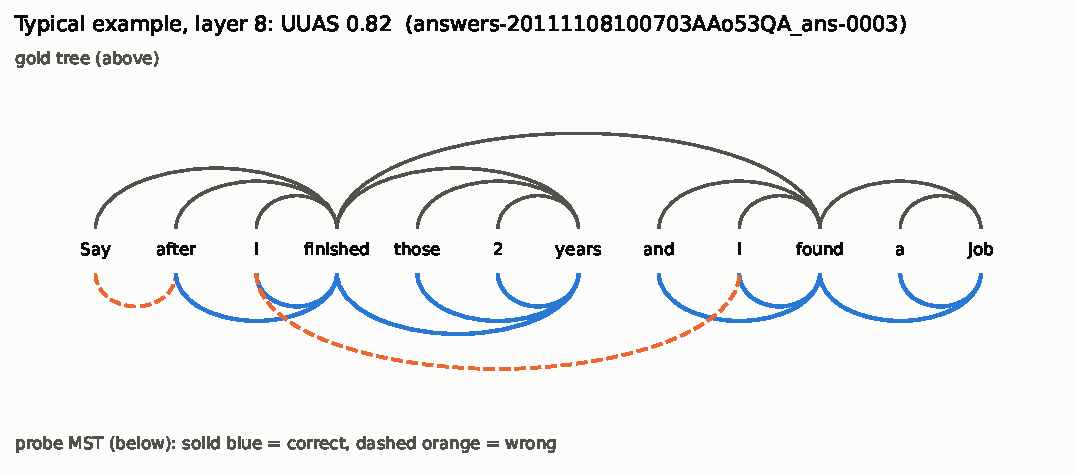
\includegraphics[width=0.62\textwidth]{example_typical.pdf}\\[2pt]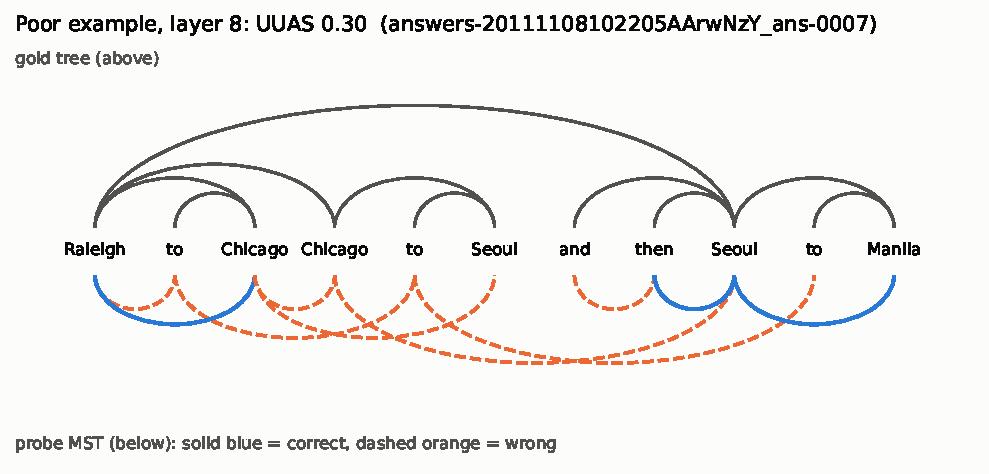
\includegraphics[width=0.62\textwidth]{example_poor.pdf}
\caption{A's probe (layer 8) on the median and worst 10--18-word test sentences. Gold tree above, probe MST below (blue = correct, orange dashed = wrong).}
\label{fig:t2ex}\end{figure}

\blk{Task 3 analogies (A, Table~\ref{tab:analogy})}
\begin{itemize}
\item \textbf{Successes:} near-perfect on regular morphology (plural \TThreePlural\%) and frequent capitals (\TThreeCapital\%).
\item \textbf{Failures:} currency (\TThreeCurrency; ``real'' is always an adjective in EWT train).
\item \textbf{Near misses:} a semantic neighbour beats the morphological target (cooler $\to$ nicer, biggest $\to$ largest) -- the same substitute bias.
\item \textbf{One representative sentence} of A's 20 (Fig.~\ref{fig:mstex}, appendix): T1 and T3 get \ExTOne\%, raw contextual vectors
\ExCtx\%, the probe \ExProbe\%; the T3 tree is a star around ``a'' and ``of''.
\end{itemize}
\begin{table}[h]\centering\footnotesize\setlength{\tabcolsep}{4pt}\begin{tabular}{llll}
\toprule
section & question ($a:b::c:$\,\textbf{gold}) & T3 answer & T1 answer \\
\midrule
capital-common-countries & baghdad : iraq :: beijing : \textbf{china} & china \checkmark & jintao \\
capital-world & amman : jordan :: baghdad : \textbf{iraq} & iraq \checkmark & threats \\
city-in-state & houston : texas :: philadelphia : \textbf{pennsylvania} & pennsylvania \checkmark & franchise \\
family & boy : girl :: brother : \textbf{sister} & sister \checkmark & cousin \\
gram1-adjective-to-adverb & amazing : amazingly :: complete : \textbf{completely} & completely \checkmark & digest \\
gram2-opposite & acceptable : unacceptable :: aware : \textbf{unaware} & unaware \checkmark & socially \\
\midrule
capital-world & beijing : china :: kingston : \textbf{jamaica} & jamaican & northwest \\
currency & brazil : real :: canada : \textbf{dollar} & actual & church \\
gram2-opposite & acceptable : unacceptable :: certain : \textbf{uncertain} & specific & socially \\
gram3-comparative & bad : worse :: cool : \textbf{cooler} & nicer & dried \\
gram4-superlative & bad : worst :: big : \textbf{biggest} & largest & chinese \\
gram6-nationality-adjective & australia : australian :: england : \textbf{english} & british & soper \\
\bottomrule
\end{tabular}

\caption{A: analogy questions T3 solves and T1 does not (top) and T3 failures (bottom).}\label{tab:analogy}\end{table}

% =====================================================================================================
\needspace{11\baselineskip}\section{Discussion}\label{sec:disc}
\blk{What the comparison adds}
\begin{itemize}
\item Two independent implementations make the main claims much stronger: the best syntax layer, the T3 semantic gain, the T3 structural
failure, the disagreement between the evaluations and the best static layers are all reproduced.
\item The Task~3 numbers match exactly once settings are aligned.
\item \textbf{Three choices change numbers by more than the effects being studied} -- reports should state them explicitly:
\begin{enumerate}
\item the probe's learning-rate schedule (11--18\pt{} UUAS; it also flips the best rank);
\item the evaluation subset (248 vs.\ 203 covered pairs move T1's $\rho$ from 0.10 to 0.17--0.19; the MST sample moves the baselines by up to 8\pt);
\item the OOV imputation rule for ``all 353'' (0.048 vs.\ 0.060 for A's own vectors).
\end{enumerate}
\end{itemize}
\blk{What worked / what did not}
\begin{itemize}
\item \textbf{Worked:} the probe reproduces the paper when its schedule is reproduced; pooled BERT vectors are strong lexical vectors; one
post-processing step (centring or all-but-the-top) helps.
\item \textbf{Did not work:} PPMI-SVD on 200k words cannot do analogies; pooling from the \emph{syntax} layer does not produce
\emph{syntactic} static vectors -- the semantic benchmarks measure similarity between word types, while trees are relations between tokens
in context, which pooling removes.
\end{itemize}
\blk{Limitations}
\begin{itemize}
\item B's numbers are transcribed from B's report (no raw outputs); B's DSpr/NSpr definitions differ slightly from A's.
\item Each probe was trained once; the two MST samples differ.
\item BERT vs.\ PPMI is not a data-matched comparison; one treebank.
\end{itemize}

% =====================================================================================================
\needspace{11\baselineskip}\section{Reproducibility}\label{sec:repro}
\begin{itemize}
\item \textbf{A:} \texttt{SEED=42} (Python, NumPy, PyTorch) for the sample, baselines, bootstraps and SVD; probe seed $42+1000\ell+k$ (+500 depth);
pinned EWT tag, gensim commit and model revision \texttt{86b5e09}; \texttt{python code/run\_all.py} or the Colab notebook runs everything;
every number is generated from the outputs; 2$\times$L40S, 78 probes in 49+54\,min.
\item \textbf{B:} sentence-sample seed 42, SVD start vector 0, probe seed $1000k$ (+7 depth) + first layer of the chunk; EWT \texttt{.conllu}
files; Task~1 in about 13\,s on CPU.
\item \textbf{Code:} \url{https://github.com/trishitasaha/NLP_Assignment2} -- B at the root (\texttt{Codes/}, \texttt{results/}), A in
\texttt{23CS10081\_Yellapu\_Dheeraj\_Babu/}, this report in \texttt{Combined/}.
\item \textbf{Deviations from the specification:}
\begin{itemize}
\item both: best-dev checkpoint selection; \lstar{} chosen on dev, not test; WS-353 and analogies reported on covered and on all items;
the 20-sentence check complemented by a larger set;
\item A only: the paper's lr decay (justified by the control in \S\ref{sec:t2}); layer 0 probed; punctuation excluded from the structural check.
\end{itemize}
\end{itemize}

\FloatBarrier
\begin{thebibliography}{99}\setlength{\itemsep}{0pt}\small
\bibitem[Bommasani et~al.(2020)]{bommasani} R.~Bommasani, K.~Davis, C.~Cardie. Interpreting pretrained contextualized representations via reductions to static embeddings. \emph{ACL}, 2020.
\bibitem[de~Marneffe et~al.(2021)]{ud} M.-C.~de~Marneffe, C.~D.~Manning, J.~Nivre, D.~Zeman. Universal Dependencies. \emph{Computational Linguistics} 47(2), 2021.
\bibitem[Devlin et~al.(2019)]{devlin} J.~Devlin, M.-W.~Chang, K.~Lee, K.~Toutanova. BERT: pre-training of deep bidirectional transformers for language understanding. \emph{NAACL}, 2019.
\bibitem[Ethayarajh(2019)]{ethayarajh} K.~Ethayarajh. How contextual are contextualized word representations? \emph{EMNLP}, 2019.
\bibitem[Finkelstein et~al.(2002)]{ws353} L.~Finkelstein et~al. Placing search in context: the concept revisited. \emph{ACM TOIS} 20(1), 2002.
\bibitem[Hewitt and Manning(2019)]{hewitt} J.~Hewitt, C.~D.~Manning. A structural probe for finding syntax in word representations. \emph{NAACL}, 2019.
\bibitem[Levy and Goldberg(2014)]{levy2014} O.~Levy, Y.~Goldberg. Neural word embedding as implicit matrix factorization. \emph{NeurIPS}, 2014.
\bibitem[Levy et~al.(2015)]{levy2015} O.~Levy, Y.~Goldberg, I.~Dagan. Improving distributional similarity with lessons learned from word embeddings. \emph{TACL} 3, 2015.
\bibitem[Mikolov et~al.(2013)]{mikolov} T.~Mikolov, K.~Chen, G.~Corrado, J.~Dean. Efficient estimation of word representations in vector space. \emph{ICLR Workshop}, 2013.
\bibitem[Mu and Viswanath(2018)]{mu} J.~Mu, P.~Viswanath. All-but-the-top: simple and effective postprocessing for word representations. \emph{ICLR}, 2018.
\bibitem[Sahlgren(2006)]{sahlgren} M.~Sahlgren. \emph{The Word-Space Model}. PhD thesis, Stockholm University, 2006.
\bibitem[Silveira et~al.(2014)]{silveira} N.~Silveira et~al. A gold standard dependency corpus for English. \emph{LREC}, 2014.
\end{thebibliography}

\clearpage
\appendix
\section{Additional material (implementation A)}
\begin{figure}[H]\centering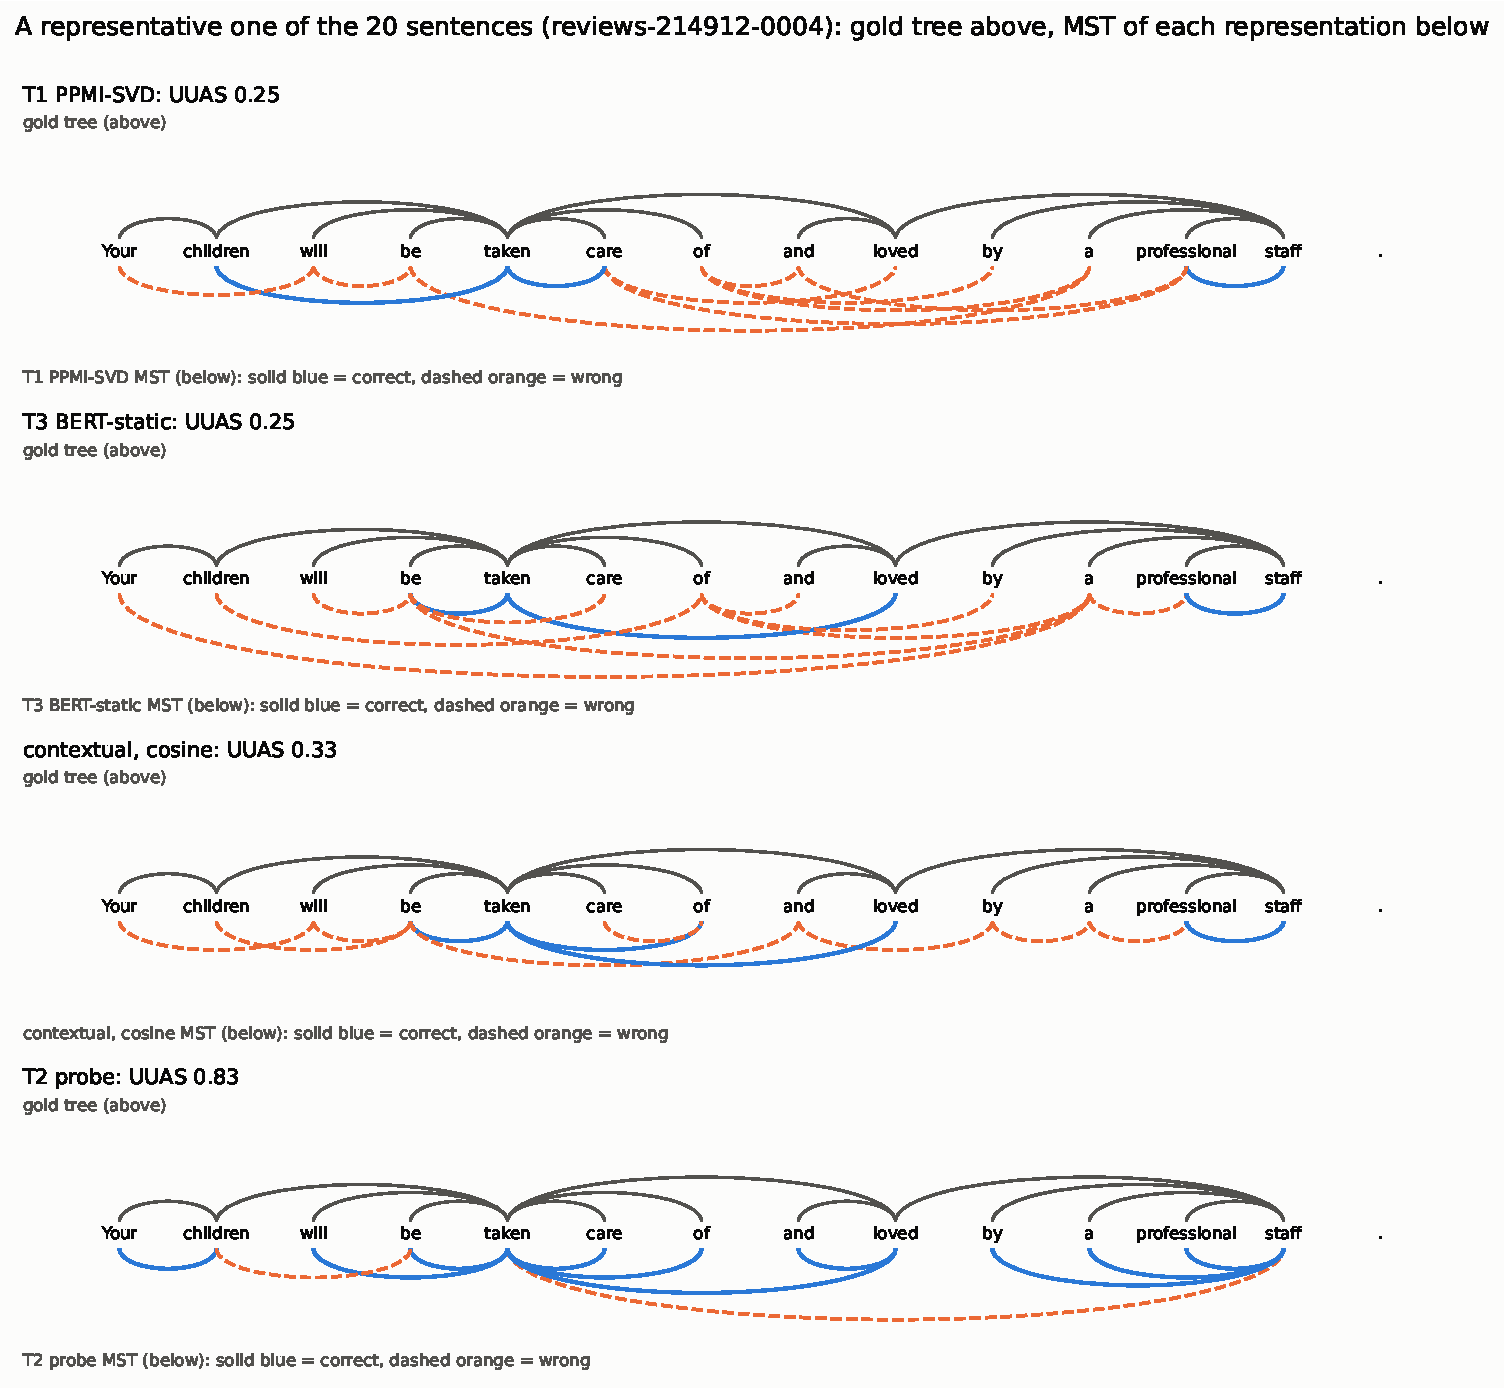
\includegraphics[width=0.80\textwidth]{mst_example.pdf}
\caption{``\ExText'' -- gold tree (above) and the MST of each representation (below), implementation A.}\label{fig:mstex}\end{figure}
\begin{table}[H]\centering\footnotesize\setlength{\tabcolsep}{4pt}\begin{tabular}{rccccccccc}
\toprule
 & \multicolumn{2}{c}{WS-353 $\rho$ (cov.)} & \multicolumn{2}{c}{Analogy (cov., \%)} & \multicolumn{4}{c}{MST UUAS on the pool (\%)} & \\
\cmidrule(lr){2-3}\cmidrule(lr){4-5}\cmidrule(lr){6-9}
$\ell$ & raw & ABTT & raw & ABTT & static raw & static ABTT & contextual cos. & T2 probe & anisotropy \\
\midrule
0 & 0.685 & 0.703 & 72.1 & 69.4 & 17.0 & 16.4 & 23.2 & 63.8 & 0.04 \\
1 & 0.690 & 0.686 & 75.9 & 74.0 & 16.7 & 17.0 & 24.6 & 71.1 & 0.09 \\
2 & 0.675 & 0.693 & 80.3 & 79.7 & 15.4 & 17.3 & 24.0 & 73.3 & 0.13 \\
3 & 0.658 & 0.682 & 78.0 & 78.3 & 15.6 & 16.9 & 23.9 & 77.9 & 0.16 \\
4 & 0.602 & 0.644 & 77.1 & 77.6 & 15.9 & 17.2 & 26.7 & 82.3 & 0.21 \\
5 & 0.587 & 0.645 & 74.1 & 75.4 & 15.3 & 17.3 & 28.3 & 83.1 & 0.25 \\
6 & 0.578 & 0.647 & 72.3 & 73.7 & 15.5 & 17.6 & 30.7 & 83.8 & 0.27 \\
7 & 0.577 & 0.666 & 70.4 & 73.0 & 16.4 & 18.2 & 34.1 & 83.6 & 0.28 \\
\rowcolor{black!8} 8 & 0.577 & 0.682 & 67.7 & 71.0 & 17.9 & 19.6 & 38.2 & 82.9 & 0.29 \\
9 & 0.592 & 0.713 & 66.1 & 69.2 & 19.2 & 20.1 & 38.8 & 79.4 & 0.29 \\
10 & 0.552 & 0.711 & 62.9 & 67.5 & 19.8 & 20.5 & 37.4 & 75.0 & 0.32 \\
11 & 0.488 & 0.706 & 62.1 & 68.2 & 19.0 & 20.8 & 36.5 & 72.3 & 0.40 \\
12 & 0.528 & 0.691 & 63.7 & 69.0 & 18.9 & 20.2 & 34.4 & 70.5 & 0.33 \\
\midrule
T1 & 0.104 & 0.153 & 0.5 & 0.4 & 24.8 & 24.5 & -- & -- & 0.12 \\
\bottomrule
\end{tabular}

\caption{A's layer sweep in numbers (covered items; pool = 660 sentences).}\end{table}
\begin{figure}[H]\centering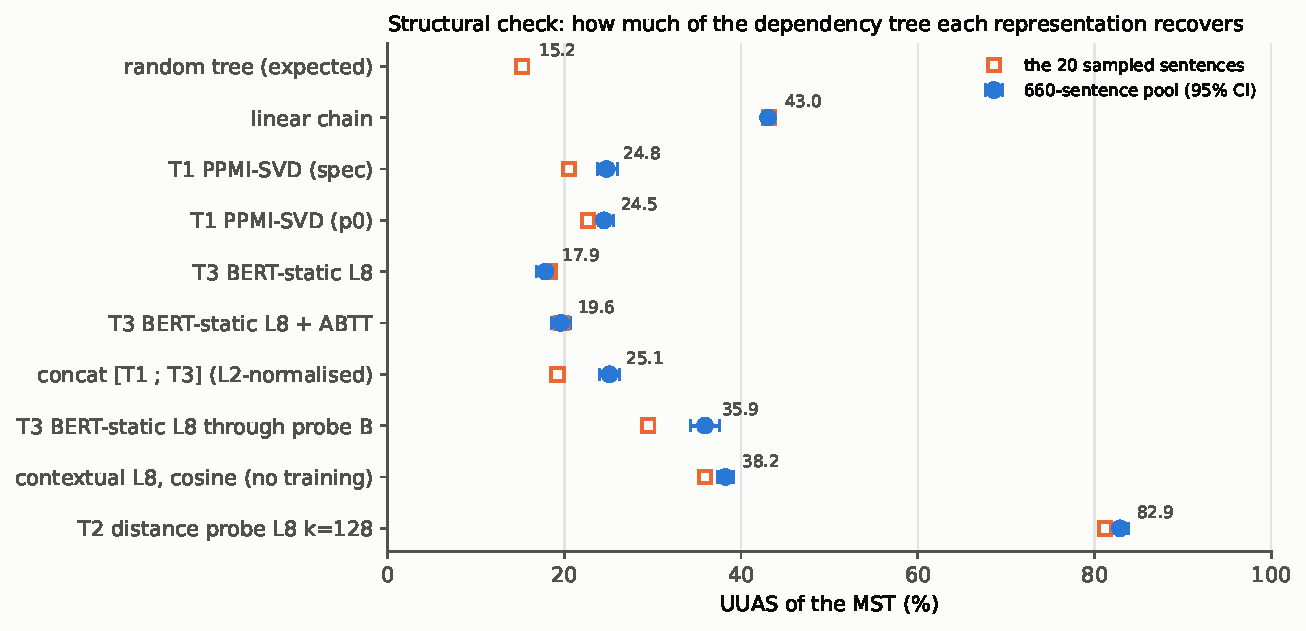
\includegraphics[width=0.80\textwidth]{ladder.pdf}
\caption{A's diagnostic ladder: MST UUAS on the 660-sentence pool (95\% CI) and on the 20 sentences.}\end{figure}
\end{document}
